\documentclass{article}
\usepackage[utf8]{inputenc}

\title{Final Exam Problem 2 }
\author{Yuancheng Xu}
\date{Dec 17, 2020}

% Optional math commands from https://github.com/goodfeli/dlbook_notation.
%%%%% NEW MATH DEFINITIONS %%%%%

\usepackage{amsmath,amsfonts,bm}

% Mark sections of captions for referring to divisions of figures
\newcommand{\figleft}{{\em (Left)}}
\newcommand{\figcenter}{{\em (Center)}}
\newcommand{\figright}{{\em (Right)}}
\newcommand{\figtop}{{\em (Top)}}
\newcommand{\figbottom}{{\em (Bottom)}}
\newcommand{\captiona}{{\em (a)}}
\newcommand{\captionb}{{\em (b)}}
\newcommand{\captionc}{{\em (c)}}
\newcommand{\captiond}{{\em (d)}}

% Highlight a newly defined term
\newcommand{\newterm}[1]{{\bf #1}}


% Figure reference, lower-case.
\def\figref#1{figure~\ref{#1}}
% Figure reference, capital. For start of sentence
\def\Figref#1{Figure~\ref{#1}}
\def\twofigref#1#2{figures \ref{#1} and \ref{#2}}
\def\quadfigref#1#2#3#4{figures \ref{#1}, \ref{#2}, \ref{#3} and \ref{#4}}
% Section reference, lower-case.
\def\secref#1{section~\ref{#1}}
% Section reference, capital.
\def\Secref#1{Section~\ref{#1}}
% Reference to two sections.
\def\twosecrefs#1#2{sections \ref{#1} and \ref{#2}}
% Reference to three sections.
\def\secrefs#1#2#3{sections \ref{#1}, \ref{#2} and \ref{#3}}
% Reference to an equation, lower-case.
\def\eqref#1{equation~\ref{#1}}
% Reference to an equation, upper case
\def\Eqref#1{Equation~\ref{#1}}
% A raw reference to an equation---avoid using if possible
\def\plaineqref#1{\ref{#1}}
% Reference to a chapter, lower-case.
\def\chapref#1{chapter~\ref{#1}}
% Reference to an equation, upper case.
\def\Chapref#1{Chapter~\ref{#1}}
% Reference to a range of chapters
\def\rangechapref#1#2{chapters\ref{#1}--\ref{#2}}
% Reference to an algorithm, lower-case.
\def\algref#1{algorithm~\ref{#1}}
% Reference to an algorithm, upper case.
\def\Algref#1{Algorithm~\ref{#1}}
\def\twoalgref#1#2{algorithms \ref{#1} and \ref{#2}}
\def\Twoalgref#1#2{Algorithms \ref{#1} and \ref{#2}}
% Reference to a part, lower case
\def\partref#1{part~\ref{#1}}
% Reference to a part, upper case
\def\Partref#1{Part~\ref{#1}}
\def\twopartref#1#2{parts \ref{#1} and \ref{#2}}

\def\ceil#1{\lceil #1 \rceil}
\def\floor#1{\lfloor #1 \rfloor}
\def\1{\bm{1}}
\newcommand{\train}{\mathcal{D}}
\newcommand{\valid}{\mathcal{D_{\mathrm{valid}}}}
\newcommand{\test}{\mathcal{D_{\mathrm{test}}}}

\def\eps{{\epsilon}}


% Random variables
\def\reta{{\textnormal{$\eta$}}}
\def\ra{{\textnormal{a}}}
\def\rb{{\textnormal{b}}}
\def\rc{{\textnormal{c}}}
\def\rd{{\textnormal{d}}}
\def\re{{\textnormal{e}}}
\def\rf{{\textnormal{f}}}
\def\rg{{\textnormal{g}}}
\def\rh{{\textnormal{h}}}
\def\ri{{\textnormal{i}}}
\def\rj{{\textnormal{j}}}
\def\rk{{\textnormal{k}}}
\def\rl{{\textnormal{l}}}
% rm is already a command, just don't name any random variables m
\def\rn{{\textnormal{n}}}
\def\ro{{\textnormal{o}}}
\def\rp{{\textnormal{p}}}
\def\rq{{\textnormal{q}}}
\def\rr{{\textnormal{r}}}
\def\rs{{\textnormal{s}}}
\def\rt{{\textnormal{t}}}
\def\ru{{\textnormal{u}}}
\def\rv{{\textnormal{v}}}
\def\rw{{\textnormal{w}}}
\def\rx{{\textnormal{x}}}
\def\ry{{\textnormal{y}}}
\def\rz{{\textnormal{z}}}

% Random vectors
\def\rvepsilon{{\mathbf{\epsilon}}}
\def\rvtheta{{\mathbf{\theta}}}
\def\rva{{\mathbf{a}}}
\def\rvb{{\mathbf{b}}}
\def\rvc{{\mathbf{c}}}
\def\rvd{{\mathbf{d}}}
\def\rve{{\mathbf{e}}}
\def\rvf{{\mathbf{f}}}
\def\rvg{{\mathbf{g}}}
\def\rvh{{\mathbf{h}}}
\def\rvu{{\mathbf{i}}}
\def\rvj{{\mathbf{j}}}
\def\rvk{{\mathbf{k}}}
\def\rvl{{\mathbf{l}}}
\def\rvm{{\mathbf{m}}}
\def\rvn{{\mathbf{n}}}
\def\rvo{{\mathbf{o}}}
\def\rvp{{\mathbf{p}}}
\def\rvq{{\mathbf{q}}}
\def\rvr{{\mathbf{r}}}
\def\rvs{{\mathbf{s}}}
\def\rvt{{\mathbf{t}}}
\def\rvu{{\mathbf{u}}}
\def\rvv{{\mathbf{v}}}
\def\rvw{{\mathbf{w}}}
\def\rvx{{\mathbf{x}}}
\def\rvy{{\mathbf{y}}}
\def\rvz{{\mathbf{z}}}

% Elements of random vectors
\def\erva{{\textnormal{a}}}
\def\ervb{{\textnormal{b}}}
\def\ervc{{\textnormal{c}}}
\def\ervd{{\textnormal{d}}}
\def\erve{{\textnormal{e}}}
\def\ervf{{\textnormal{f}}}
\def\ervg{{\textnormal{g}}}
\def\ervh{{\textnormal{h}}}
\def\ervi{{\textnormal{i}}}
\def\ervj{{\textnormal{j}}}
\def\ervk{{\textnormal{k}}}
\def\ervl{{\textnormal{l}}}
\def\ervm{{\textnormal{m}}}
\def\ervn{{\textnormal{n}}}
\def\ervo{{\textnormal{o}}}
\def\ervp{{\textnormal{p}}}
\def\ervq{{\textnormal{q}}}
\def\ervr{{\textnormal{r}}}
\def\ervs{{\textnormal{s}}}
\def\ervt{{\textnormal{t}}}
\def\ervu{{\textnormal{u}}}
\def\ervv{{\textnormal{v}}}
\def\ervw{{\textnormal{w}}}
\def\ervx{{\textnormal{x}}}
\def\ervy{{\textnormal{y}}}
\def\ervz{{\textnormal{z}}}

% Random matrices
\def\rmA{{\mathbf{A}}}
\def\rmB{{\mathbf{B}}}
\def\rmC{{\mathbf{C}}}
\def\rmD{{\mathbf{D}}}
\def\rmE{{\mathbf{E}}}
\def\rmF{{\mathbf{F}}}
\def\rmG{{\mathbf{G}}}
\def\rmH{{\mathbf{H}}}
\def\rmI{{\mathbf{I}}}
\def\rmJ{{\mathbf{J}}}
\def\rmK{{\mathbf{K}}}
\def\rmL{{\mathbf{L}}}
\def\rmM{{\mathbf{M}}}
\def\rmN{{\mathbf{N}}}
\def\rmO{{\mathbf{O}}}
\def\rmP{{\mathbf{P}}}
\def\rmQ{{\mathbf{Q}}}
\def\rmR{{\mathbf{R}}}
\def\rmS{{\mathbf{S}}}
\def\rmT{{\mathbf{T}}}
\def\rmU{{\mathbf{U}}}
\def\rmV{{\mathbf{V}}}
\def\rmW{{\mathbf{W}}}
\def\rmX{{\mathbf{X}}}
\def\rmY{{\mathbf{Y}}}
\def\rmZ{{\mathbf{Z}}}

% Elements of random matrices
\def\ermA{{\textnormal{A}}}
\def\ermB{{\textnormal{B}}}
\def\ermC{{\textnormal{C}}}
\def\ermD{{\textnormal{D}}}
\def\ermE{{\textnormal{E}}}
\def\ermF{{\textnormal{F}}}
\def\ermG{{\textnormal{G}}}
\def\ermH{{\textnormal{H}}}
\def\ermI{{\textnormal{I}}}
\def\ermJ{{\textnormal{J}}}
\def\ermK{{\textnormal{K}}}
\def\ermL{{\textnormal{L}}}
\def\ermM{{\textnormal{M}}}
\def\ermN{{\textnormal{N}}}
\def\ermO{{\textnormal{O}}}
\def\ermP{{\textnormal{P}}}
\def\ermQ{{\textnormal{Q}}}
\def\ermR{{\textnormal{R}}}
\def\ermS{{\textnormal{S}}}
\def\ermT{{\textnormal{T}}}
\def\ermU{{\textnormal{U}}}
\def\ermV{{\textnormal{V}}}
\def\ermW{{\textnormal{W}}}
\def\ermX{{\textnormal{X}}}
\def\ermY{{\textnormal{Y}}}
\def\ermZ{{\textnormal{Z}}}

% Vectors
\def\vzero{{\bm{0}}}
\def\vone{{\bm{1}}}
\def\vmu{{\bm{\mu}}}
\def\vtheta{{\bm{\theta}}}
\def\va{{\bm{a}}}
\def\vb{{\bm{b}}}
\def\vc{{\bm{c}}}
\def\vd{{\bm{d}}}
\def\ve{{\bm{e}}}
\def\vf{{\bm{f}}}
\def\vg{{\bm{g}}}
\def\vh{{\bm{h}}}
\def\vi{{\bm{i}}}
\def\vj{{\bm{j}}}
\def\vk{{\bm{k}}}
\def\vl{{\bm{l}}}
\def\vm{{\bm{m}}}
\def\vn{{\bm{n}}}
\def\vo{{\bm{o}}}
\def\vp{{\bm{p}}}
\def\vq{{\bm{q}}}
\def\vr{{\bm{r}}}
\def\vs{{\bm{s}}}
\def\vt{{\bm{t}}}
\def\vu{{\bm{u}}}
\def\vv{{\bm{v}}}
\def\vw{{\bm{w}}}
\def\vx{{\bm{x}}}
\def\vy{{\bm{y}}}
\def\vz{{\bm{z}}}

% Elements of vectors
\def\evalpha{{\alpha}}
\def\evbeta{{\beta}}
\def\evepsilon{{\epsilon}}
\def\evlambda{{\lambda}}
\def\evomega{{\omega}}
\def\evmu{{\mu}}
\def\evpsi{{\psi}}
\def\evsigma{{\sigma}}
\def\evtheta{{\theta}}
\def\eva{{a}}
\def\evb{{b}}
\def\evc{{c}}
\def\evd{{d}}
\def\eve{{e}}
\def\evf{{f}}
\def\evg{{g}}
\def\evh{{h}}
\def\evi{{i}}
\def\evj{{j}}
\def\evk{{k}}
\def\evl{{l}}
\def\evm{{m}}
\def\evn{{n}}
\def\evo{{o}}
\def\evp{{p}}
\def\evq{{q}}
\def\evr{{r}}
\def\evs{{s}}
\def\evt{{t}}
\def\evu{{u}}
\def\evv{{v}}
\def\evw{{w}}
\def\evx{{x}}
\def\evy{{y}}
\def\evz{{z}}

% Matrix
\def\mA{{\bm{A}}}
\def\mB{{\bm{B}}}
\def\mC{{\bm{C}}}
\def\mD{{\bm{D}}}
\def\mE{{\bm{E}}}
\def\mF{{\bm{F}}}
\def\mG{{\bm{G}}}
\def\mH{{\bm{H}}}
\def\mI{{\bm{I}}}
\def\mJ{{\bm{J}}}
\def\mK{{\bm{K}}}
\def\mL{{\bm{L}}}
\def\mM{{\bm{M}}}
\def\mN{{\bm{N}}}
\def\mO{{\bm{O}}}
\def\mP{{\bm{P}}}
\def\mQ{{\bm{Q}}}
\def\mR{{\bm{R}}}
\def\mS{{\bm{S}}}
\def\mT{{\bm{T}}}
\def\mU{{\bm{U}}}
\def\mV{{\bm{V}}}
\def\mW{{\bm{W}}}
\def\mX{{\bm{X}}}
\def\mY{{\bm{Y}}}
\def\mZ{{\bm{Z}}}
\def\mBeta{{\bm{\beta}}}
\def\mPhi{{\bm{\Phi}}}
\def\mLambda{{\bm{\Lambda}}}
\def\mSigma{{\bm{\Sigma}}}

% Tensor
\DeclareMathAlphabet{\mathsfit}{\encodingdefault}{\sfdefault}{m}{sl}
\SetMathAlphabet{\mathsfit}{bold}{\encodingdefault}{\sfdefault}{bx}{n}
\newcommand{\tens}[1]{\bm{\mathsfit{#1}}}
\def\tA{{\tens{A}}}
\def\tB{{\tens{B}}}
\def\tC{{\tens{C}}}
\def\tD{{\tens{D}}}
\def\tE{{\tens{E}}}
\def\tF{{\tens{F}}}
\def\tG{{\tens{G}}}
\def\tH{{\tens{H}}}
\def\tI{{\tens{I}}}
\def\tJ{{\tens{J}}}
\def\tK{{\tens{K}}}
\def\tL{{\tens{L}}}
\def\tM{{\tens{M}}}
\def\tN{{\tens{N}}}
\def\tO{{\tens{O}}}
\def\tP{{\tens{P}}}
\def\tQ{{\tens{Q}}}
\def\tR{{\tens{R}}}
\def\tS{{\tens{S}}}
\def\tT{{\tens{T}}}
\def\tU{{\tens{U}}}
\def\tV{{\tens{V}}}
\def\tW{{\tens{W}}}
\def\tX{{\tens{X}}}
\def\tY{{\tens{Y}}}
\def\tZ{{\tens{Z}}}


% Graph
\def\gA{{\mathcal{A}}}
\def\gB{{\mathcal{B}}}
\def\gC{{\mathcal{C}}}
\def\gD{{\mathcal{D}}}
\def\gE{{\mathcal{E}}}
\def\gF{{\mathcal{F}}}
\def\gG{{\mathcal{G}}}
\def\gH{{\mathcal{H}}}
\def\gI{{\mathcal{I}}}
\def\gJ{{\mathcal{J}}}
\def\gK{{\mathcal{K}}}
\def\gL{{\mathcal{L}}}
\def\gM{{\mathcal{M}}}
\def\gN{{\mathcal{N}}}
\def\gO{{\mathcal{O}}}
\def\gP{{\mathcal{P}}}
\def\gQ{{\mathcal{Q}}}
\def\gR{{\mathcal{R}}}
\def\gS{{\mathcal{S}}}
\def\gT{{\mathcal{T}}}
\def\gU{{\mathcal{U}}}
\def\gV{{\mathcal{V}}}
\def\gW{{\mathcal{W}}}
\def\gX{{\mathcal{X}}}
\def\gY{{\mathcal{Y}}}
\def\gZ{{\mathcal{Z}}}

% Sets
\def\sA{{\mathbb{A}}}
\def\sB{{\mathbb{B}}}
\def\sC{{\mathbb{C}}}
\def\sD{{\mathbb{D}}}
% Don't use a set called E, because this would be the same as our symbol
% for expectation.
\def\sF{{\mathbb{F}}}
\def\sG{{\mathbb{G}}}
\def\sH{{\mathbb{H}}}
\def\sI{{\mathbb{I}}}
\def\sJ{{\mathbb{J}}}
\def\sK{{\mathbb{K}}}
\def\sL{{\mathbb{L}}}
\def\sM{{\mathbb{M}}}
\def\sN{{\mathbb{N}}}
\def\sO{{\mathbb{O}}}
\def\sP{{\mathbb{P}}}
\def\sQ{{\mathbb{Q}}}
\def\sR{{\mathbb{R}}}
\def\sS{{\mathbb{S}}}
\def\sT{{\mathbb{T}}}
\def\sU{{\mathbb{U}}}
\def\sV{{\mathbb{V}}}
\def\sW{{\mathbb{W}}}
\def\sX{{\mathbb{X}}}
\def\sY{{\mathbb{Y}}}
\def\sZ{{\mathbb{Z}}}

% Entries of a matrix
\def\emLambda{{\Lambda}}
\def\emA{{A}}
\def\emB{{B}}
\def\emC{{C}}
\def\emD{{D}}
\def\emE{{E}}
\def\emF{{F}}
\def\emG{{G}}
\def\emH{{H}}
\def\emI{{I}}
\def\emJ{{J}}
\def\emK{{K}}
\def\emL{{L}}
\def\emM{{M}}
\def\emN{{N}}
\def\emO{{O}}
\def\emP{{P}}
\def\emQ{{Q}}
\def\emR{{R}}
\def\emS{{S}}
\def\emT{{T}}
\def\emU{{U}}
\def\emV{{V}}
\def\emW{{W}}
\def\emX{{X}}
\def\emY{{Y}}
\def\emZ{{Z}}
\def\emSigma{{\Sigma}}

% entries of a tensor
% Same font as tensor, without \bm wrapper
\newcommand{\etens}[1]{\mathsfit{#1}}
\def\etLambda{{\etens{\Lambda}}}
\def\etA{{\etens{A}}}
\def\etB{{\etens{B}}}
\def\etC{{\etens{C}}}
\def\etD{{\etens{D}}}
\def\etE{{\etens{E}}}
\def\etF{{\etens{F}}}
\def\etG{{\etens{G}}}
\def\etH{{\etens{H}}}
\def\etI{{\etens{I}}}
\def\etJ{{\etens{J}}}
\def\etK{{\etens{K}}}
\def\etL{{\etens{L}}}
\def\etM{{\etens{M}}}
\def\etN{{\etens{N}}}
\def\etO{{\etens{O}}}
\def\etP{{\etens{P}}}
\def\etQ{{\etens{Q}}}
\def\etR{{\etens{R}}}
\def\etS{{\etens{S}}}
\def\etT{{\etens{T}}}
\def\etU{{\etens{U}}}
\def\etV{{\etens{V}}}
\def\etW{{\etens{W}}}
\def\etX{{\etens{X}}}
\def\etY{{\etens{Y}}}
\def\etZ{{\etens{Z}}}

% The true underlying data generating distribution
\newcommand{\pdata}{p_{\rm{data}}}
% The empirical distribution defined by the training set
\newcommand{\ptrain}{\hat{p}_{\rm{data}}}
\newcommand{\Ptrain}{\hat{P}_{\rm{data}}}
% The model distribution
\newcommand{\pmodel}{p_{\rm{model}}}
\newcommand{\Pmodel}{P_{\rm{model}}}
\newcommand{\ptildemodel}{\tilde{p}_{\rm{model}}}
% Stochastic autoencoder distributions
\newcommand{\pencode}{p_{\rm{encoder}}}
\newcommand{\pdecode}{p_{\rm{decoder}}}
\newcommand{\precons}{p_{\rm{reconstruct}}}

\newcommand{\laplace}{\mathrm{Laplace}} % Laplace distribution

\newcommand{\E}{\mathbb{E}}
\newcommand{\Ls}{\mathcal{L}}
\newcommand{\R}{\mathbb{R}}
\newcommand{\emp}{\tilde{p}}
\newcommand{\lr}{\alpha}
\newcommand{\reg}{\lambda}
\newcommand{\rect}{\mathrm{rectifier}}
\newcommand{\softmax}{\mathrm{softmax}}
\newcommand{\sigmoid}{\sigma}
\newcommand{\softplus}{\zeta}
\newcommand{\KL}{D_{\mathrm{KL}}}
\newcommand{\Var}{\mathrm{Var}}
\newcommand{\standarderror}{\mathrm{SE}}
\newcommand{\Cov}{\mathrm{Cov}}
% Wolfram Mathworld says $L^2$ is for function spaces and $\ell^2$ is for vectors
% But then they seem to use $L^2$ for vectors throughout the site, and so does
% wikipedia.
\newcommand{\normlzero}{L^0}
\newcommand{\normlone}{L^1}
\newcommand{\normltwo}{L^2}
\newcommand{\normlp}{L^p}
\newcommand{\normmax}{L^\infty}

\newcommand{\parents}{Pa} % See usage in notation.tex. Chosen to match Daphne's book.

\DeclareMathOperator*{\argmax}{arg\,max}
\DeclareMathOperator*{\argmin}{arg\,min}

\DeclareMathOperator{\sign}{sign}
\DeclareMathOperator{\Tr}{Tr}
\let\ab\allowbreak


\usepackage{natbib}
\usepackage{amsmath}
\usepackage{bm}
\usepackage{multirow}
\usepackage{amssymb}
\usepackage{hyperref}
\usepackage{url}
\usepackage{enumerate}
\usepackage{bbm}
\usepackage{graphicx}
\usepackage{pdfpages}
\usepackage{amsthm}
% \usepackage{subfigure} % cannot use with "subcaption package"

% \DeclareMathOperator{\Tr}{Tr}

\newtheorem{theorem}{Theorem}[section]
\newtheorem{corollary}{Corollary}[theorem]
\newtheorem{lemma}[theorem]{Lemma}
\usepackage{subcaption}



\begin{document}

\maketitle

%\noindent Code link:\\
%\url{https://github.com/Yuancheng-Xu/AMSC-808N/tree/master/HW6}\\

\section*{Q1}
Firstly, we give an expression for the critical transmissibility $ T_c $. As derived in class, we have $ T_c =  \frac{\sum_{k=1}^{\infty}kp_k}{\sum_{k=1}^{\infty}k(k-1)p_k} = \frac{\langle k \rangle}{\langle k^2 \rangle - \langle k \rangle} = \frac{1}{\kappa - 1}$. Note that since the original graph has a giant component, $ \kappa > 2 $ and thus $ T_c <1 $.

Now assume that $ T > T_c $ (so there will be an epidemic if we do nothing) and we would like to know  if we vaccinate a fraction $ v $ of randomly selected nodes (before the spread of disease), can we destroy the epidemic and most importantly, what is the critical value $ v_c $ (the minimal fraction of vaccinated node in order to stop the epidemic). Taking the vaccine into account and assuming there is no epidemic, we will first derive the generating function for the transmitting edges, then the generating function for the size of transmitting cluster and finally, the average outbreak size, from which we will extract the critical $ v_c $.

As usual, let $ G_0(x) = \sum_{k=0}^{\infty}p_k x^k $ and $ G_1(x) =\frac{G_0'(x)}{\langle k \rangle} $ denote the generating function for degree and excess degree distribution. Note that the probability that an edge is transmitting, when taking the vaccine into account, is $ (1-v)T $ and is not transmitting with probability $ v + (1-v)(1-T) $. Therefore, the generating function for distribution of transmitting edges adjacent to a node is 

\begin{equation}\label{G_0}
	\begin{aligned}
		G_0(x;T) & = \sum_{m=0}^{\infty}\sum_{k=m}^{\infty}p_k \binom{k}{m}((1-v)T)^m (v+(1-v)(1-T))^{k-m}x^m \\
		& = \sum_{k=0}^{\infty}p_k\sum_{m=0}^{k} \binom{k}{m}((1-v)Tx)^m (v+(1-v)(1-T))^{k-m}\\
		& = \sum_{k=0}^{\infty}p_k ((1-v)Tx + v+(1-v)(1-T) )^k \\ 
		& = G_0((1-v)Tx + 1 - T + Tv)
	\end{aligned}
\end{equation}

Similarly, we can obtain the generating function for distribution of transmitting edges adjacent to a node arrived at by a randomly chosen edge

\begin{equation}\label{G_1}
	\begin{aligned}
		G_1(x;T) = G_1((1-v)Tx + 1 - T + Tv)
	\end{aligned}
\end{equation}

Then the generating functions for the size of transmitting cluster reached from a random edge and vertex are given by
\begin{equation}\label{H_1}
	H_1(x;T) = xG_1(H_1(x;T);T)
\end{equation}

\begin{equation}\label{H_0}
	H_0(x;T) = xG_0(H_1(x;T);T)
\end{equation}

By differentiating Equation \ref{G_0} and Equation \ref{G_1} and substituting $ x=1 $, we have $ G_0'(1;T) = T(1-v)G_0'(1) $ and $ G_1'(1;T) = T(1-v)G_1'(1) $. By differentiating Equation \ref{H_1} we have $ H_1'(1;T) = 1 + G_1'(1;T)H_1'(1;T) = \frac{1}{1-G_1'(1;T)} $. Finally, using Equation \ref{H_0}, we compute the average outbreak size as 

\begin{equation}\label{eq: avg outbreak size}
	\begin{aligned}
		\langle s \rangle & = H_0'(1;T) \\
		& = 1 + G_0'(1;T) H_1'(1;T) \\
		& = 1 + \frac{G_0'(1;T)}{1-G_1'(1;T)} \\
		& = 1 + \frac{T(1-v)G_0'(1)}{1 - T(1-v)G_1'(1)}
	\end{aligned}
\end{equation}

Therefore, the phase transition occurs when $ 1 - T(1-v)G_1'(1) = 0 $. Since T is given here (with $ T>T_c =  \frac{1}{\kappa - 1}$), the critical fraction of nodes $$ v_c = 1 - \frac{1}{TG_1'(1)} = 1 - \frac{T_c}{T} $$Note that $0 \leq v_c \leq 1 - T_c \leq1$. If $ v>v_c $, epidemic cannot occur and if $ v<v_c $, one may occur. 

\section*{Q2}

\subsection*{(a)}
First we compute the generating function for degree and excess degree distribution. Denote $ \mathrm{Li}_\alpha(x) =\sum_{k=1}^{\infty} \frac{x^k}{k^\alpha}$ and therefore $ \mathrm{Li}_\alpha(1) = \zeta(\alpha)$. Note that $ \mathrm{Li}_\alpha '(x) = \frac{1}{x}\mathrm{Li}_{\alpha-1}(x) $

$$ G_0(x) = \frac{1}{\mathrm{Li}_\alpha(1)}\sum_{k=1}^{\infty}k^{-\alpha}x^k = \frac{1}{\mathrm{Li}_\alpha(1)}\mathrm{Li}_\alpha(x)$$

$$ G_1(x) =\frac{G_0'(x)}{\langle k \rangle} =  \frac{\mathrm{Li}_\alpha '(x)}{\mathrm{Li}_\alpha(1) \frac{\mathrm{Li}_{\alpha-1}(1)}{\mathrm{Li}_\alpha(1)}} = \frac{\mathrm{Li}_{\alpha-1}(x)}{x\mathrm{Li}_{\alpha-1}(1)}$$

Now let $ u $ be the solution of $ u = G_1(u) $ (we  numerically compute $ u $ by solving $ u =   \frac{\mathrm{Li}_{\alpha-1}(u)}{u\mathrm{Li}_{\alpha-1}(1)}$ in Matlab). As we have derived in class, the fraction $ S $ of nodes in the giant component can be computed by $ S = 1 - G_0(u) $. Therefore, $$ S = 1 - \frac{\mathrm{Li}_\alpha(u)}{\mathrm{Li}_\alpha(1)} $$.

Using $ \alpha = 2.2 $ , we find $ u = 0.1963 $ and $ S = 0.8622 $, which is the fraction of nodes in the giant component.

\subsection*{(b)}
As derived in the slides, denote $ u = H_1(1;T) $ and we have $ u = G_1(u;T) = G_1(1+(u-1)T) $. Therefore, we numerically solve $$ u =  \frac{\mathrm{Li}_{\alpha-1}(1+(u-1)T)}{(1+(u-1)T)\mathrm{Li}_{\alpha-1}(1)}$$

Then we compute the fraction $ S(T) $ of nodes affected by the epidemic (the fraction of the giant component) as $ S(T) = 1 - H_0(1;T) $ where $ H_0(1;T) = G_0(u;T) =  G_0(1+(u-1)T) = \frac{\mathrm{Li}_\alpha(1+(u-1)T)}{\mathrm{Li}_\alpha(1)} $. That is, $$ S(T) = 1 - \frac{\mathrm{Li}_\alpha(1+(u-1)T)}{\mathrm{Li}_\alpha(1)} $$

Using $ \alpha=2.2, T=0.4 $, we have $ u =  0.2883 $ and $ S(T) = 0.4078
 $, which is the fraction of nodes affected by the epidemic if it occurs. 

\subsection*{(c)}
As derived in Question 1, $$v_c = 1 - \frac{T_c}{T} $$ where  $ T_c =    \frac{1}{\kappa - 1}$. The first moment $ \langle k \rangle = \frac{\mathrm{Li}_{\alpha-1}(1)}{\mathrm{Li}_{\alpha}(1)}$ and the second moment  $ \langle k^2 \rangle = \frac{1}{\mathrm{Li}_\alpha(1)}\sum_{k=1}^{\infty}k^2 k^{-\alpha} $ does not exist (since $ \alpha<3 $),  and thus formally $ \kappa = \infty $, $ T_c = 0 $.

Therefore, the critical fraction $ v_c $ to vaccinate is $ v_c = 1 $ (vaccinate everyone), for any $ T>0 $.

\section*{Q3}
In this question, we will run numerical simulations and compare the results with those in Q2. 

\subsection*{(a)}
We use DFS to find the size of the gaint component. Note that the theoretical value for an infinite graph is $ S = 0.8622 $.

The value obtained by simulation is $ 0.8211 $, averaged over 100 runs.

\subsection*{(b)} 
To simulate this, we first generate the original graph and then keep each edge with probability $ T $. Then we use DFS to find the size of the giant component if there is one, which corresponds to the fraction of nodes affected by an epidemic. Note that the theoretical value for an infinite graph is $ S_T = 0.4078 $.

The value obtained by simulation is $ 0.3691 $, averaged over 100 runs.

\subsection*{(c)}
Since $ \alpha < 3 $, by theory we have $ T_c =0 $ for an infinite graph. Therefore, by theory, as long as $ T>0 $, the giant component (epidemic) occurs. To verify if this is true in the simulation, we plot the fraction $ S $ versus $ T $ in Figure \ref{fig: Q3_c}. By printing out specific values in this figure, we observe that when $ T<0.03 $, we find $ S<0.01 $ and $ S $ increases slowly with $ T $. Therefore we suspect that $ T_c = 0.03 $ is the critical value for this finite graph (so below this threshold there is no giant component). When $ T>0.03 $, $ S $ is roughly linear in $ T $ and epidemic obviously occurs.

\begin{figure}[htp]
	\centering
	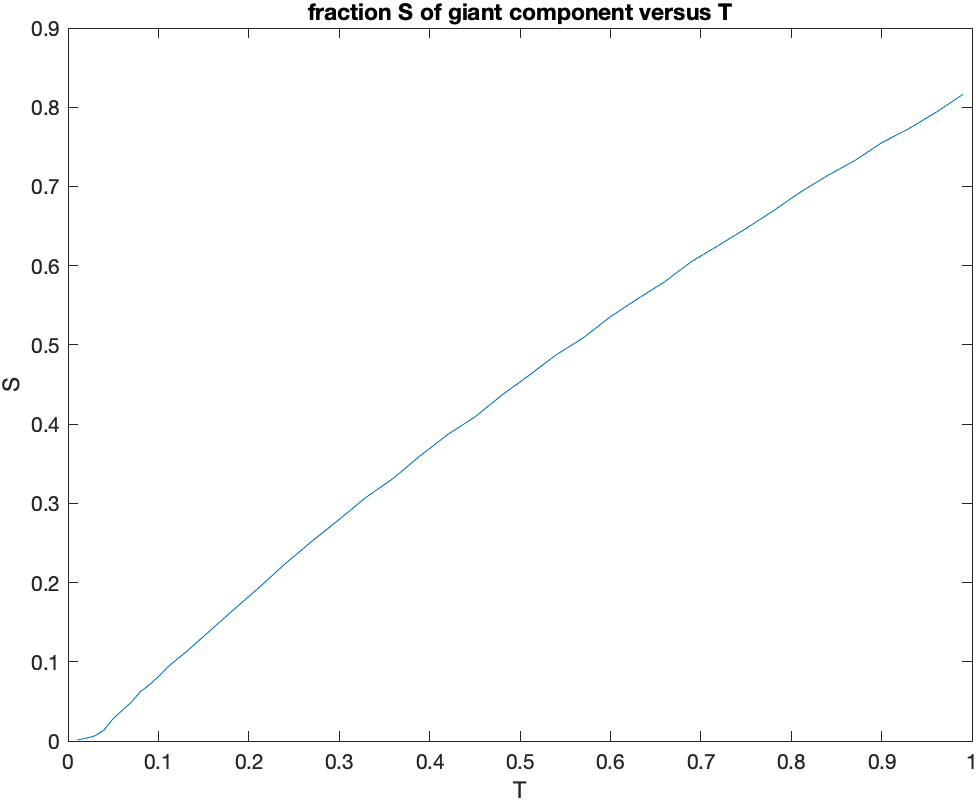
\includegraphics[width=.8\linewidth]{figs/Q3_c.png}
	\caption{fraction $ S $ of the giant component (the fraction affected by an epidemic) versus $ T $. For each $ T $ value, $ S $ is averaged over 20 runs.}
	\label{fig: Q3_c}
\end{figure}

\subsection*{(d)}
As we have seen in Q2, the critical value $ v_c = 1 $ by theory. To simulate this, we first generate the original graph and vaccinate fraction $ v $ of nodes. Then for each edge in the original graph, if the corresponding node is not vaccinated, then with probability $ T $ we keep it and otherwise, we remove it. We run DFS on the resulting graph to obtain the fraction of the giant component.

The result is shown in Figure \ref{fig: Q3_d}. We see that as expected, the fraction $ S $ decreases as vaccine $ v $ increases. However, in order to fully eliminate the epidemic (say, $ S < 0.01 $), we need $ v >  0.93 $ and therefore we conclude that in this finite graph case, $ v_c = 0.93 $ (this is also observed by printing out the values in Figure \ref{fig: Q3_d}).

\begin{figure}[htp]
	\centering
	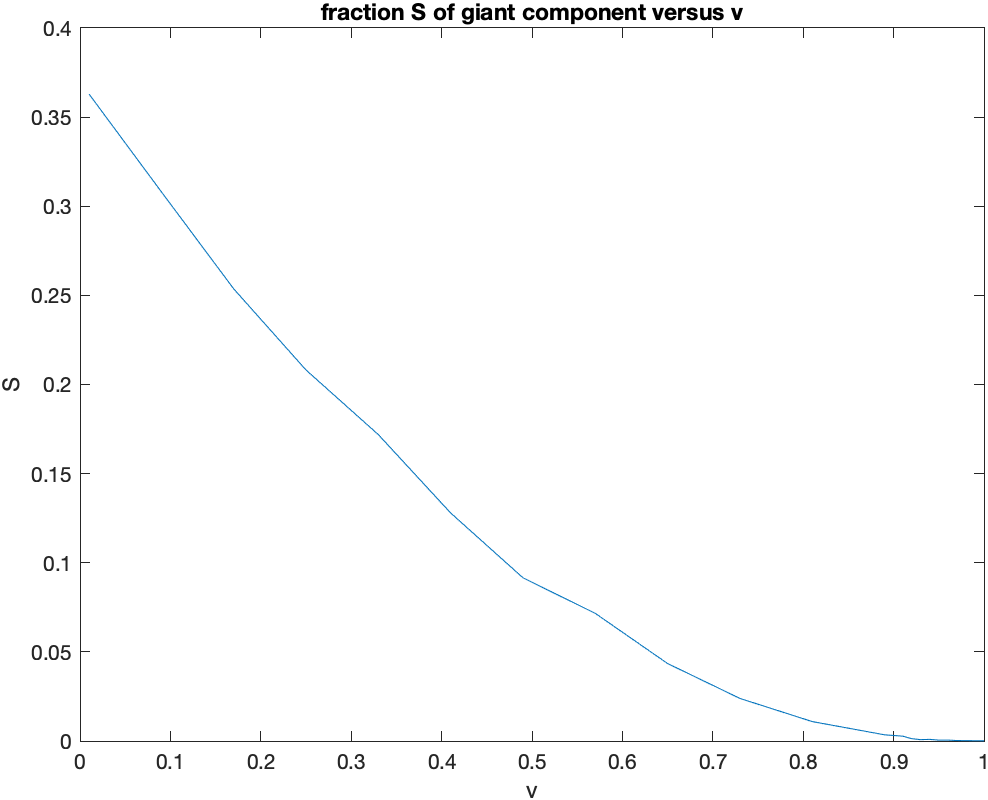
\includegraphics[width=.8\linewidth]{figs/Q3_d.png}
	\caption{fraction $ S $ of the giant component (the fraction affected by an epidemic) versus $ v $, with $ T = 0.4 $. For each $ v $ value, $ S $ is averaged over 20 runs.}
	\label{fig: Q3_d}
\end{figure}

\section*{Q4}
Here we run a discrete time SIR model (with $ \alpha=2.2, T = 0.4 $ and no vaccine) from a single infecting node. We assume that each infecting node remains infecting for one time step (for example, at time $ t-1 $, a node v is uninfected; at time $ t $, it is infected. Then it is infecting at $ t+1 $ and not infecting at $ t+2 $ ). The epidemic graph is generated in the same way as in Q3.c. Note that in this question, by construction, the transmitting edges are fixed forever (in the graph generating process) while in practice, it may happen that at time $ t $ a node infects a fraction $ T $ of its neighbors and at the next time step $ t+1 $, it infects potentially a different fraction of its neighbors. However, we only focus on simulating
 the fixed transmitting edges case.
 
Using $ n = 10000$, we visualize how the fraction of infecting nodes evolves with time in Figure \ref{fig: Q4_fractionTime}. We can observe that when the epidemic does occur (when the starting infecting point is in the giant component), the fraction of infecting nodes first increases to a peak (about 0.27) and then decrease to zero.
 
 \begin{figure}[htp]
 	\centering
 	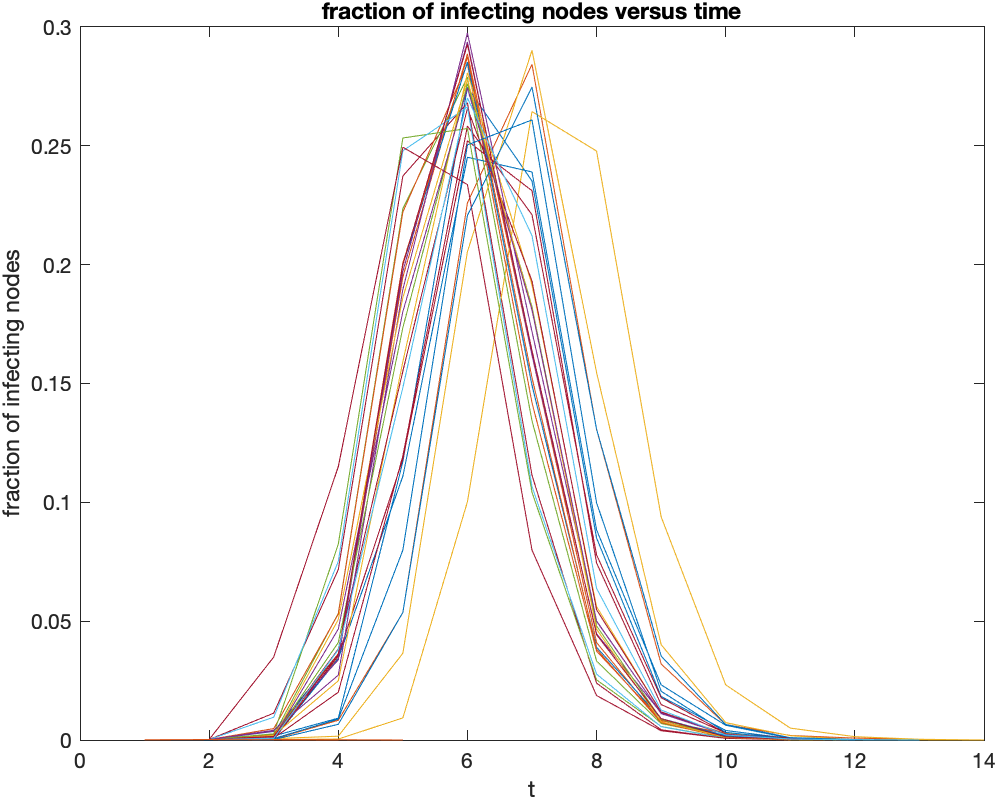
\includegraphics[width=.8\linewidth]{figs/Q4_fractionTime}
 	\caption{fraction of infecting nodes versus time $ t $. There are 100 trajectories on the graph. 31 out of 100 times, the starting point is in the giant component and therefore there is an epidemic.  Other 69 trajectories correspond to the case where the starting point is not in the giant component and therefore there is no epidemic, and these trajectories are not obvious in the figure since the fraction is almost zero and the duration is very short.  }
 	\label{fig: Q4_fractionTime}
 \end{figure}
 
\paragraph{How the duration scales with n? Relation with BFS?} 
This SIR model is very similar to Breadth-first search (BFS). Indeed, SIR can be viewed as a disease exploring the graph (after keeping edges of the original graph with probability $ T $) in a BFS manner, since at each step the disease transmit to neighbors that have never been infected (visited) before.
We would like to know how the duration scales with the number of nodes in the graph. Using the intuition of BFS, which explores the graph as if it were a tree, we can predict that the duration should scale with $ log(n) $, the height of a tree with $ n $ nodes. This is partially verified in Figure \ref{fig: Q4_duration}, where the simulations are run with varying $ n $ values. Note that only the case where the starting infecting node is in the giant component (so the epidemic occurs) is recorded.


\begin{figure} 
	\begin{subfigure}[b]{.5\linewidth}
		\centering\large 	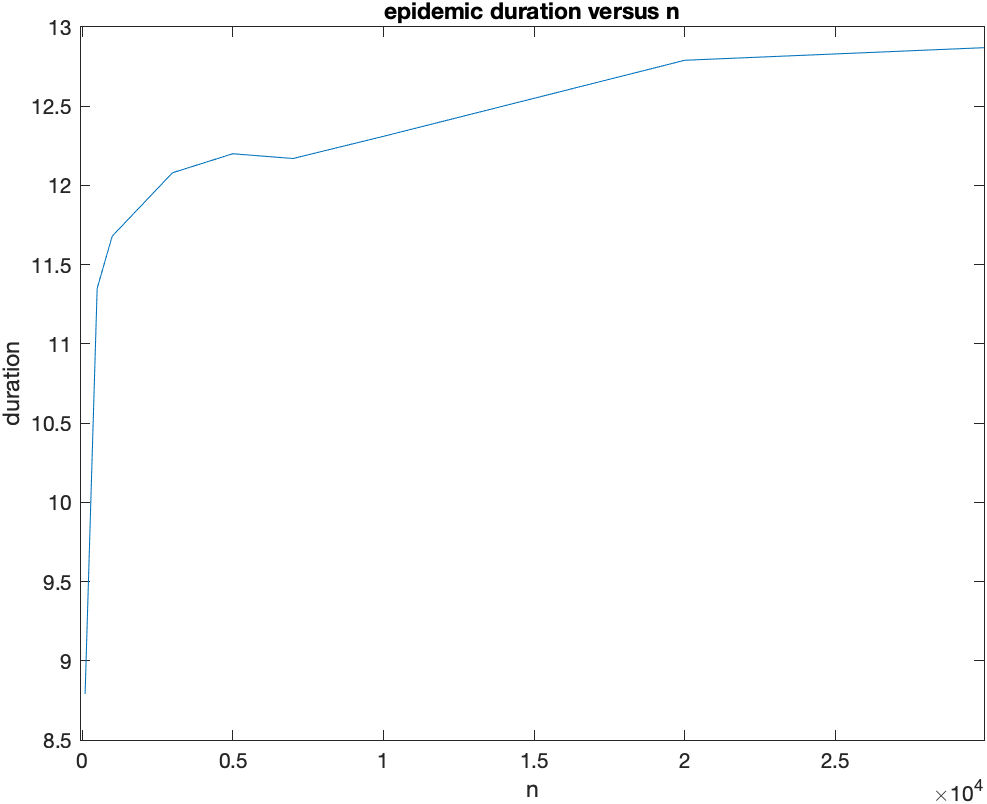
\includegraphics[width=\linewidth]{figs/Q4_duration_n.png}
		\caption{Duration VS $ n $}\label{fig: Q4_duration_1} 
	\end{subfigure}% 
	\begin{subfigure}[b]{.5\linewidth}
	\centering\large 	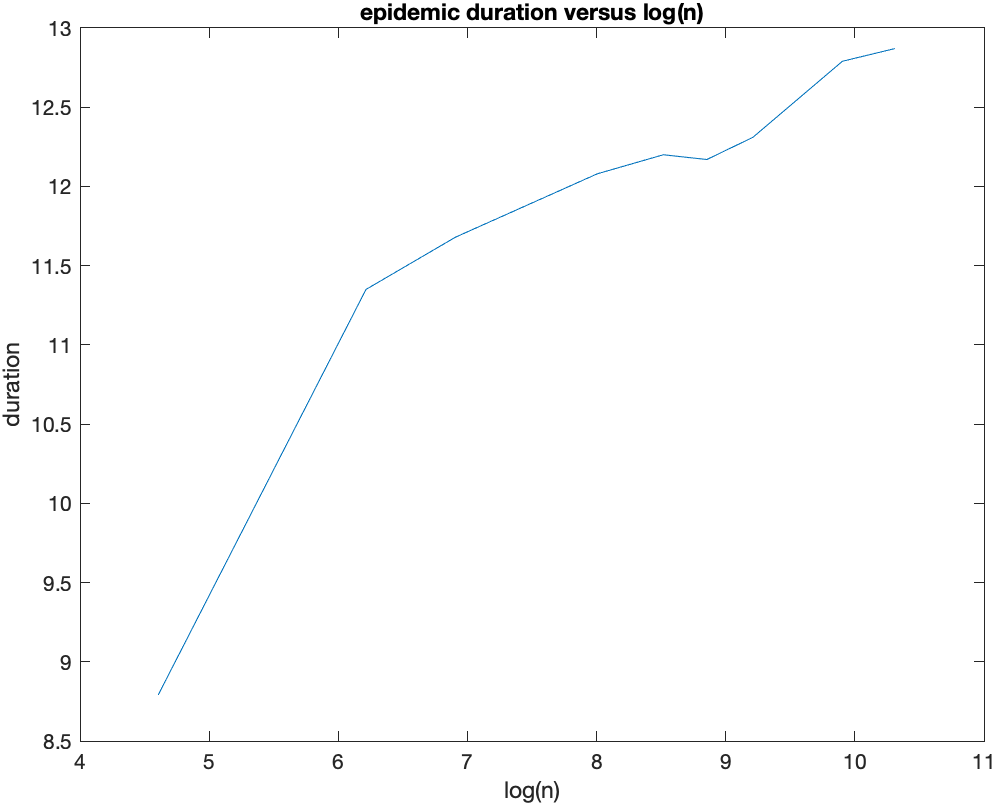
\includegraphics[width=\linewidth]{figs/Q4_duration.png}
	\caption{Duration VS $ log(n) $}\label{fig: Q4_duration_2}
	\end{subfigure}
\caption{Epidemic duration versus $ n $ and $ log(n) $. For each $ n $ value, the duration is averaged over 100 runs. We see that the duration roughly scales with $ log(n) $.}\label{fig: Q4_duration}
\end{figure}

\paragraph{Remark}
In the problem we only consider static SIR model, where all the infections happen synchronously. However, in real life, the infection may happen asynchronously, with some of paths transmit the disease much faster than the others. In that case, the SIR model is kind of a mixture of BFS and DFS. Also, in this problem we assume that an infecting node will infect all of its neighbors by transmitting edges, while in practice this will not happen. Moreover, the transmitting edges will evolve over time (since population is dynamical), in stead of static. Nevertheless, the simplified model considered in this question conveys some useful information that is potentially useful in practice.

\end{document}

				